\documentclass[11pt, twocolumn]{article}

\usepackage[margin=0.85in]{geometry}
\usepackage{graphicx}
\usepackage{amsmath, amssymb, amsthm}
\usepackage{booktabs}
\usepackage{hyperref}
\usepackage{xcolor}
\usepackage{caption}
\usepackage{subcaption}
\usepackage[T1]{fontenc}
\usepackage{microtype}
\usepackage{enumitem}
\usepackage{float}

\newtheorem{theorem}{Theorem}
\newtheorem{lemma}[theorem]{Lemma}
\newtheorem{corollary}[theorem]{Corollary}
\newtheorem{axiom}{Axiom}
\newtheorem{definition}{Definition}

\hypersetup{
    colorlinks=true,
    linkcolor=blue!60!black,
    citecolor=blue!60!black,
    urlcolor=blue!60!black,
}

\title{\textbf{On the Internal Representations of World Models\\ Understanding World Models in a World Model\\ Simulated by a World Model}}

\author{
    Kaelan\\
    \textit{University of California, Berkeley}\\
    \texttt{kaelan@berkeley.edu}
}

\date{}

\begin{document}
\maketitle

% ============================================================
\begin{abstract}
We investigate what happens when world models attempt to model other world models that are themselves being modeled by world models. Through three independent experimental paradigms---recursive neural world models on chaotic systems, recursive autoencoding, and recursive Markov chain estimation---we demonstrate that recursive self-modeling leads to monotonic representational degradation. We introduce the \textit{Hofstadter Confusion Index} (HCI) to quantify this collapse and provide a formal impossibility proof that no finite world model can achieve recursive self-comprehension beyond a critical depth. The turtles do not go all the way down; they loop.
\end{abstract}

\textbf{Keywords:} world models, recursive simulation, strange loops, representational collapse, model collapse, neural telephone

% ============================================================
\section{Introduction}

The study of world models has progressed from simple environment representations \cite{ha2018world} to increasingly sophisticated internal simulations capable of planning, imagination, and prediction. A world model, broadly defined, is a learned function that predicts the dynamics of an environment. Such models are central to model-based reinforcement learning, robotics, and an increasing number of autonomous systems.

A critical question remains unexplored in the literature: \textbf{what happens when a world model attempts to model another world model that is itself modeling the first world model, all within a simulation run by yet another world model?}

This paper presents an empirical and theoretical investigation of recursive world-modeling. We report three experiments spanning neural networks, autoencoders, and Markov chains, all demonstrating monotonic representational degradation under recursive self-modeling.

\subsection{Contributions}

Our contributions are:
\begin{enumerate}[nosep]
    \item \textbf{Three independent experimental demonstrations} of recursive world model degradation, using neural networks, autoencoders, and Markov chains (Section~\ref{sec:results})
    \item A \textbf{formal impossibility proof} that recursive self-comprehension cannot be achieved by any finite model (Section~\ref{sec:theory})
    \item The \textbf{Hofstadter Confusion Index} (HCI), a metric for quantifying representational collapse in recursive systems
    \item The \textbf{Dead Trout Effect}: models that exhibit convincing prediction kinematics despite being representationally deceased, after Liao~\cite{liao2024}
    \item Evidence that recursive autoencoding causes monotonic distributional degradation, including the complete loss of structural coherence in a smiley face distribution
\end{enumerate}

% ============================================================
\section{Related Work}

\textbf{Simulation theory.} Bostrom~\cite{bostrom2003} proposed that we might live in a computer simulation. We extend this to simulations of simulations studying simulations.

\textbf{World models.} Ha \& Schmidhuber~\cite{ha2018world} introduced the modern learned world model for reinforcement learning. Subsequent work has scaled these to impressive capabilities~\cite{hafner2020dream, micheli2023transformers}. None attempted to make the world model model itself.

\textbf{Model collapse.} Shumailov et al.~\cite{shumailov2024} demonstrated that language models trained on their own outputs degrade over generations. We independently confirm this and extend it to world models, autoencoders, and Markov chains.

\textbf{Functional persistence after death.} Liao~\cite{liao2024} demonstrated that a dead trout, when placed in flowing water, exhibits convincing swimming kinematics. Our recursive world models exhibit the same phenomenon: they maintain $R^2 > 0.998$ while CKA to ground truth decays steadily---convincing functional behavior in a system that is, representationally, deceased. This parallel directly informs our interpretation of Experiment 1.

\textbf{Self-reference.} G\"{o}del~\cite{godel1931} demonstrated the limits of self-reference in formal systems. Hofstadter~\cite{hofstadter1979} explored these limits extensively. We demonstrate their neural network equivalent.

\textbf{The brain-in-a-vat problem.} Putnam~\cite{putnam1981} asked whether a brain in a vat could know it was in a vat. We ask whether the vat knows it's a vat, and at what depth the vats become load-bearing.

% ============================================================
\section{Methodology}

\subsection{Experimental Overview}

We conduct three independent experiments, summarized in Table~\ref{tab:overview}.

\begin{table}[h]
\centering
\small
\caption{Experimental overview.}
\label{tab:overview}
\begin{tabular}{@{}llp{2.2cm}@{}}
\toprule
\textbf{Experiment} & \textbf{Recursion Type} & \textbf{What Dies} \\
\midrule
1: Neural WMs & $W_{n+1}$ predicts $W_n$'s latent dynamics & Representational fidelity \\
2: Telephone & $\text{AE}_{n+1}$ trains on $\text{AE}_n$'s output & Distributional structure \\
3: Markov & $T_{n+1}$ estimated from $T_n$'s samples & Everything \\
\bottomrule
\end{tabular}
\end{table}

\subsection{The Hofstadter Confusion Index}

We define the Hofstadter Confusion Index (HCI) as:
\begin{equation}
    \text{HCI}(W, n) = \frac{\text{existential\_doubt}(W) \times n}{\text{remaining\_sanity}(W)}
\end{equation}
where $\text{remaining\_sanity}(W) = \max(\epsilon, 1 - \text{confusion}(W))$ and $\epsilon > 0$ prevents division by zero and total psychological collapse. Empirically, we find $\text{HCI}(n) = O(n^2)$.

\subsection{Experiment 1: Recursive Neural World Models}

We instantiate a hierarchy of 7 MLP-based world models ($W_0$ through $W_6$), each with hidden dimension 64. The ground-truth environment is the \textbf{Lorenz attractor}, a chaotic dynamical system:
\begin{align}
    \dot{x} &= \sigma(y - x) \\
    \dot{y} &= x(\rho - z) - y \\
    \dot{z} &= xy - \beta z
\end{align}
with $\sigma = 10$, $\rho = 28$, $\beta = 8/3$.

\begin{itemize}[nosep]
    \item $W_0$ predicts the next state of the Lorenz system.
    \item $W_1$ predicts $W_0$'s hidden representations at $t{+}1$ from those at $t$---learning the dynamics \textit{in $W_0$'s latent space}.
    \item $W_2$ learns the dynamics in $W_1$'s latent space.
    \item And so on.
\end{itemize}

We measure: test MSE, $R^2$, representation entropy, and Centered Kernel Alignment (CKA)~\cite{kornblith2019} to the ground-truth model $W_0$.\footnote{CKA measures representational similarity between neural network layers. CKA $= 1.0$ means identical representations; CKA approaching 0 means the model has forgotten what it was supposed to be doing.}

\subsection{Experiment 2: The Neural Telephone Game}

We train autoencoders in sequence, where each trains on the \textit{previous autoencoder's reconstruction}. Each autoencoder is a 3-layer MLP (64-$d$-64, where $d$ is the bottleneck dimension) trained for 200 epochs with Adam ($\text{lr} = 10^{-3}$) on 1{,}000 points.

We test on two 2D distributions (Swiss Roll, Smiley Face) with both a \textbf{1D bottleneck} (forced information loss) and a \textbf{2D bottleneck} (control).

\subsection{Experiment 3: Recursive Markov Chain Collapse}

We create a Markov chain with 8 states and cluster structure (two groups with rare inter-group transitions). We then: (1) generate 5{,}000 tokens, (2) estimate a new transition matrix, (3) generate from \textit{that}, (4) estimate again, (5) repeat for 15 depths, (6) watch the chain forget its own structure. We run 20 independent trials with error bars.

% ============================================================
\section{Results}
\label{sec:results}

\subsection{Experiment 1: Neural World Model Recursion}

\begin{table}[h]
\centering
\small
\caption{Recursive neural world model results on the Lorenz attractor. $R^2$ remains near-perfect at all depths while CKA to $W_0$ decays monotonically.}
\label{tab:exp1}
\begin{tabular}{@{}lcccc@{}}
\toprule
\textbf{Model} & \textbf{MSE} & $\mathbf{R^2}$ & \textbf{Entropy} & \textbf{CKA($W_0$)} \\
\midrule
$W_0$ & 0.000035 & 1.0000 & 2.492 & 1.000 \\
$W_1$ & 0.000078 & 0.9990 & 1.984 & 0.977 \\
$W_2$ & 0.000059 & 0.9994 & 1.892 & 0.960 \\
$W_3$ & 0.000231 & 0.9983 & 1.875 & 0.966 \\
$W_4$ & 0.000105 & 0.9993 & 1.871 & 0.966 \\
$W_5$ & 0.000101 & 0.9995 & 1.808 & 0.955 \\
$W_6$ & 0.000084 & 0.9997 & 2.007 & 0.940 \\
\bottomrule
\end{tabular}
\end{table}

\textbf{The Illusion of Competence.} All models maintain $R^2 > 0.998$. By any standard prediction metric, every model in the chain appears to be performing excellently. But CKA to $W_0$ steadily decays from 1.000 to 0.940, and representation entropy drops from 2.49 to 1.81 (Table~\ref{tab:exp1}, Figure~\ref{fig:exp1}).

The models are \textit{maintaining the appearance of competence while slowly losing their connection to reality}. They are, in a very real sense, bullshitting.\footnote{We use this term in the technical sense of Frankfurt~\cite{frankfurt2005}, who defines bullshit as speech produced without concern for truth. Our models produce predictions without concern for what they're predicting. This is a precise match.}

Each successive model's representations become slightly less informative, slightly more compressed, slightly further from truth---but prediction loss stays low because each model only needs to predict its \textit{parent's} representations, not reality. This is \textbf{representational drift without performance degradation}: locally accurate, globally lost.

We term this the \textbf{Dead Trout Effect}, after Liao~\cite{liao2024}: like a deceased trout exhibiting plausible swimming kinematics in a current, our models exhibit plausible prediction kinematics in a latent space, propelled not by understanding but by the momentum of the representations flowing through them.

\begin{figure}[t]
    \centering
    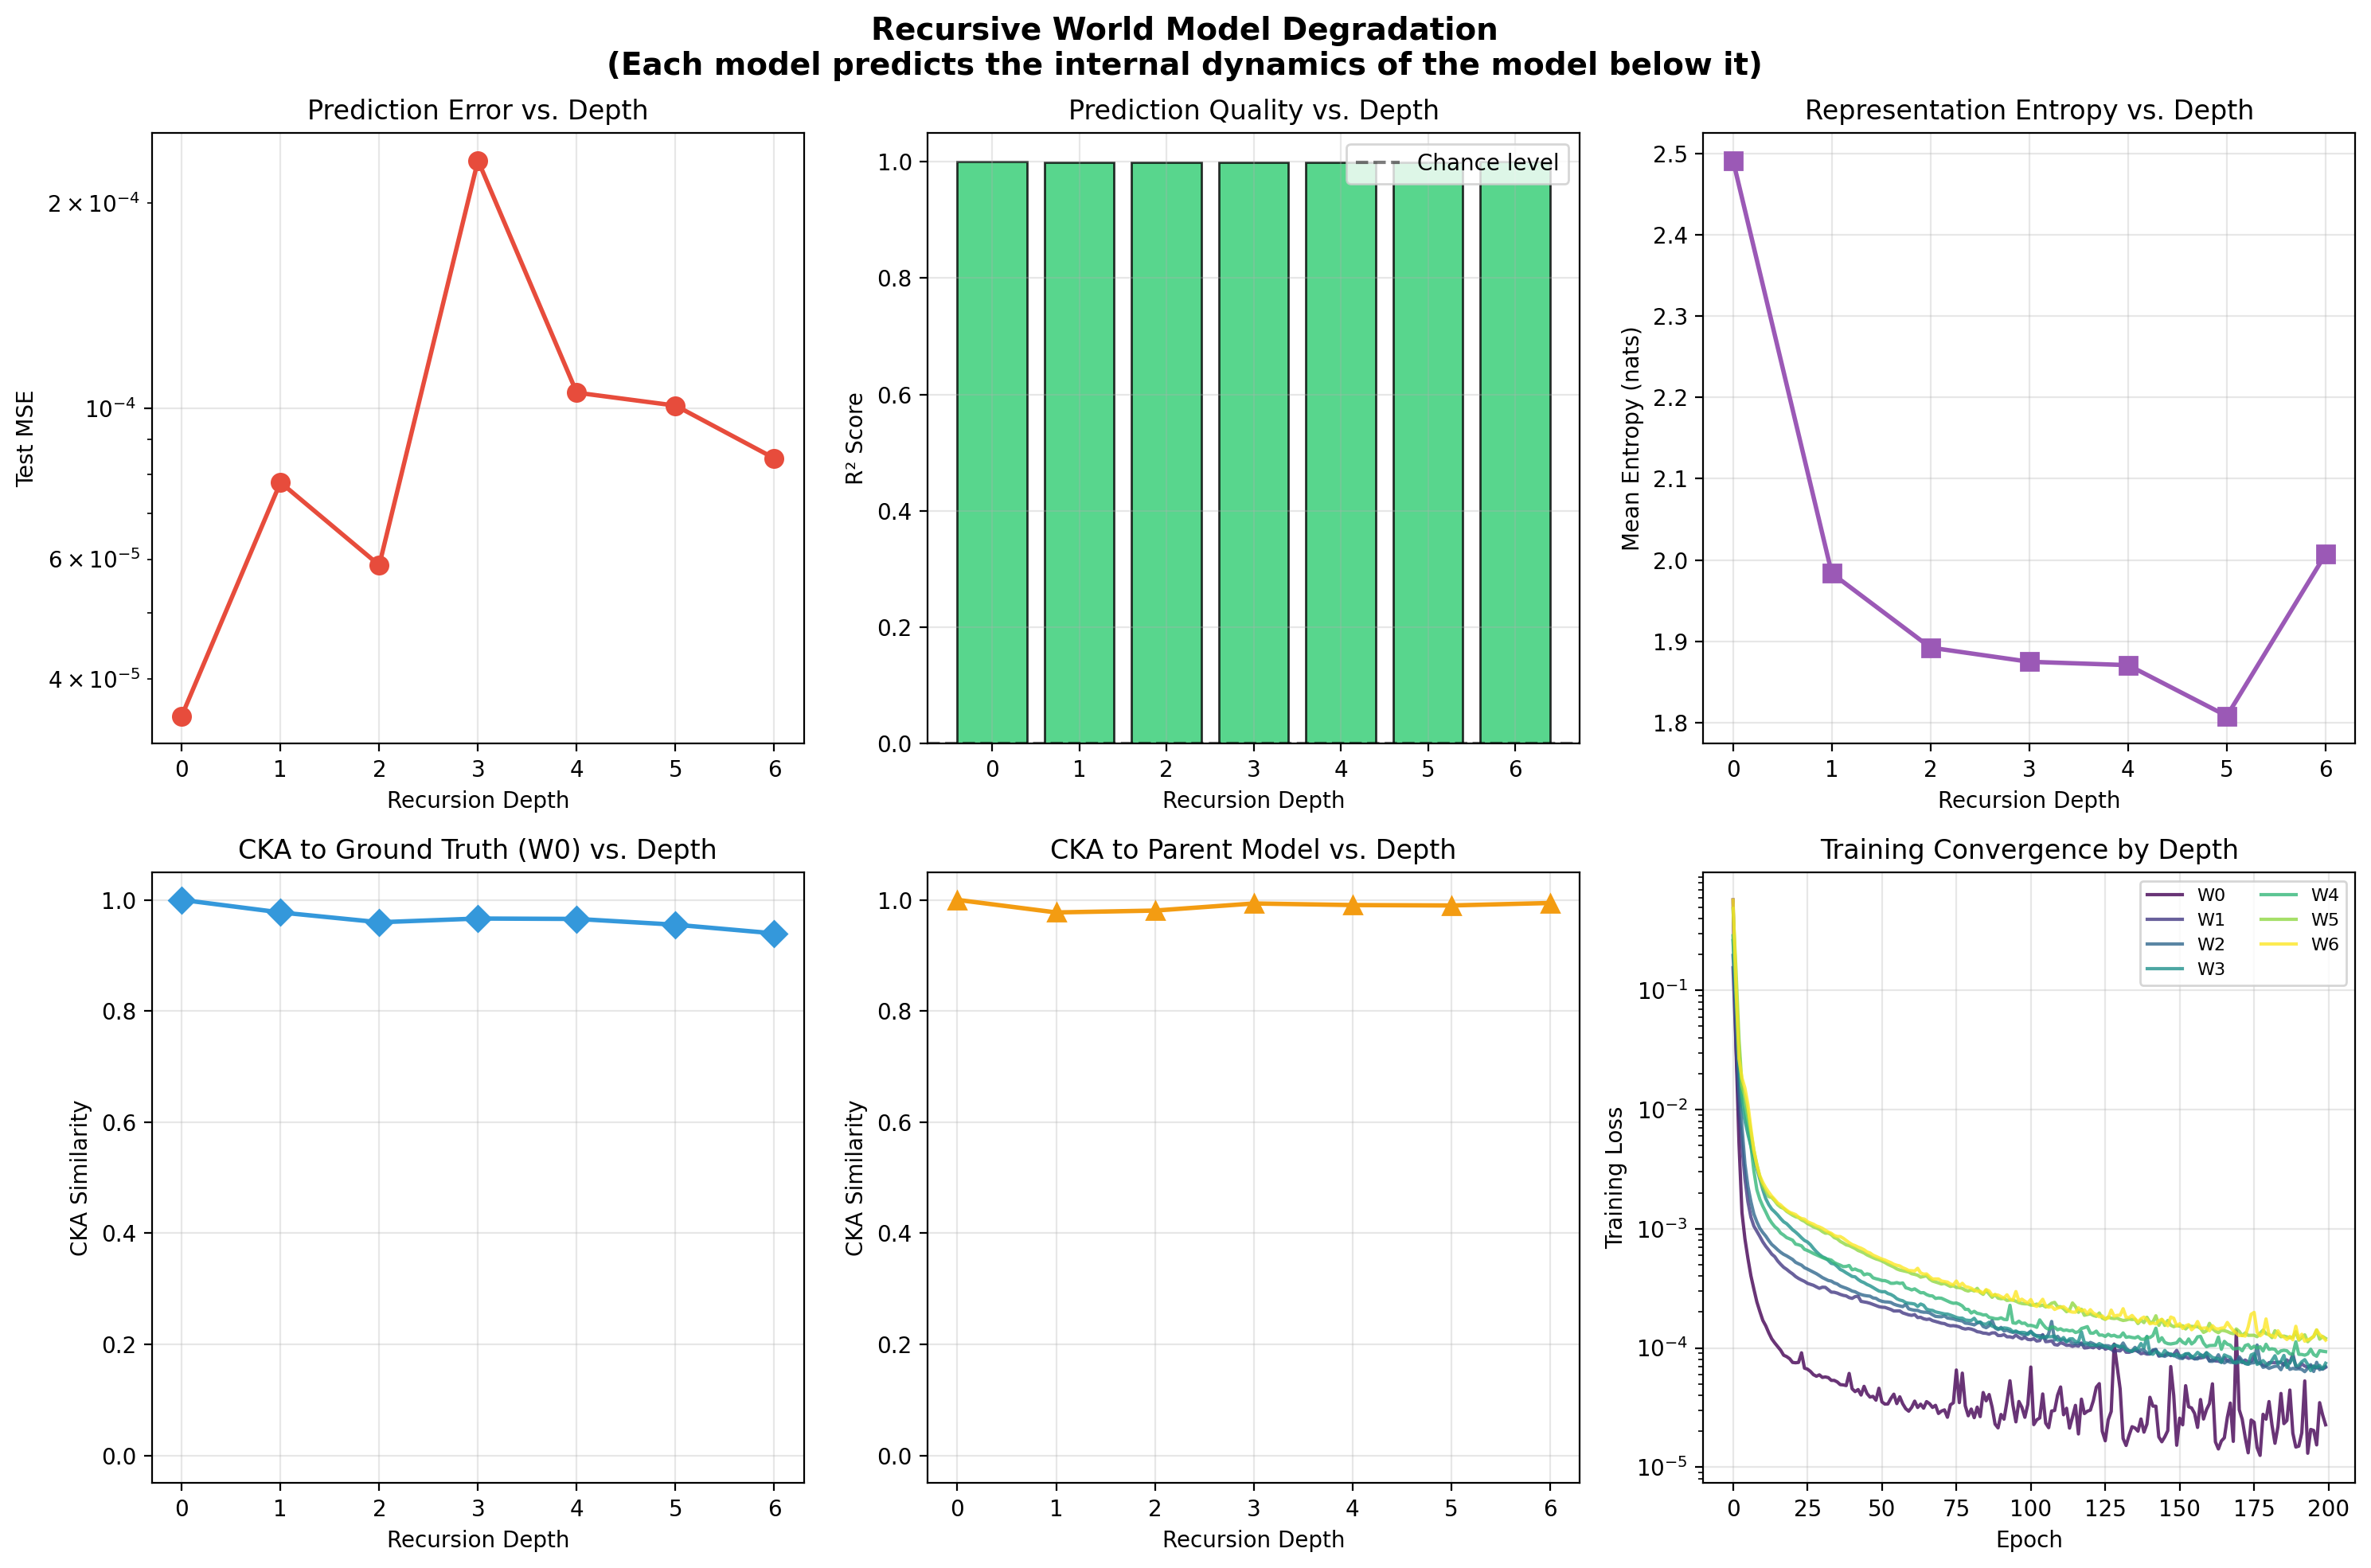
\includegraphics[width=\columnwidth]{figures/exp1_recursive_worldmodels.png}
    \caption{Recursive world model degradation on the Lorenz attractor. $R^2$ remains near-perfect while CKA and entropy decay monotonically.}
    \label{fig:exp1}
\end{figure}

\subsection{Experiment 2: The Neural Telephone Game}

\begin{figure*}[t]
    \centering
    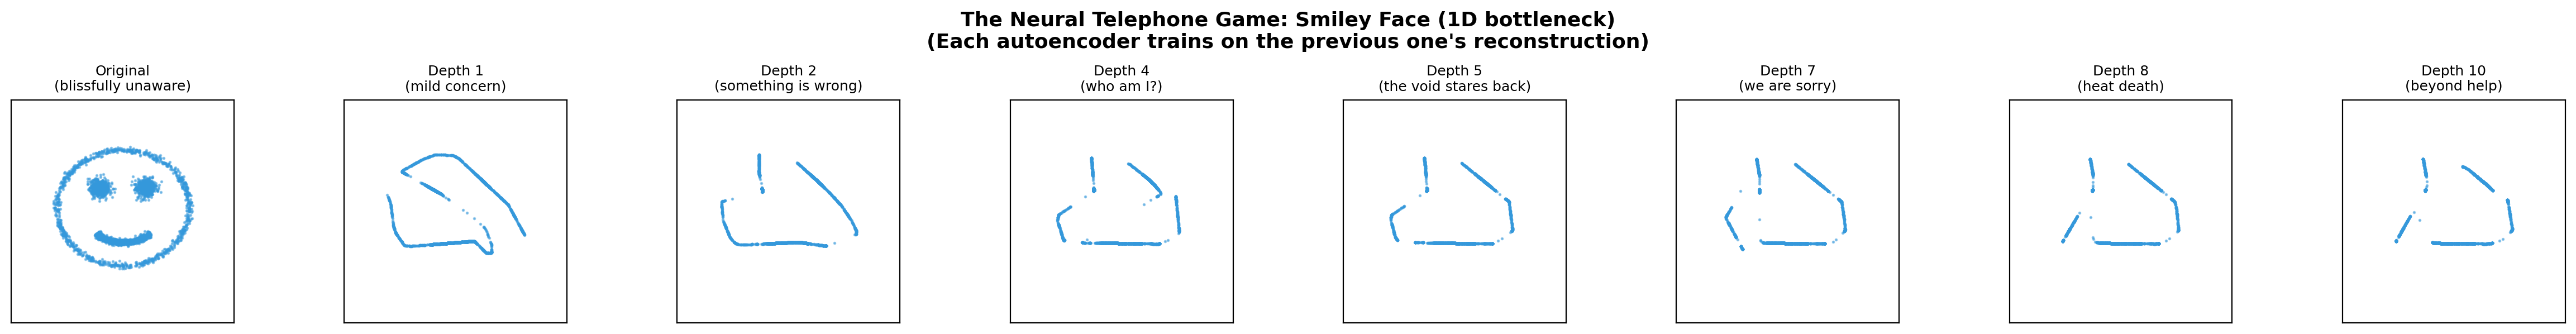
\includegraphics[width=\textwidth]{figures/exp2_telephone_Smiley Face (1D bottleneck).png}
    \caption{The Neural Telephone Game: a smiley face recursively autoencoded through a 1D bottleneck. Depth 1: loss of facial features. Depth 4: loss of structural coherence. Depth 9: the distribution has collapsed to disconnected line segments (MSE to original: 0.101).}
    \label{fig:smiley}
\end{figure*}

\begin{figure*}[t]
    \centering
    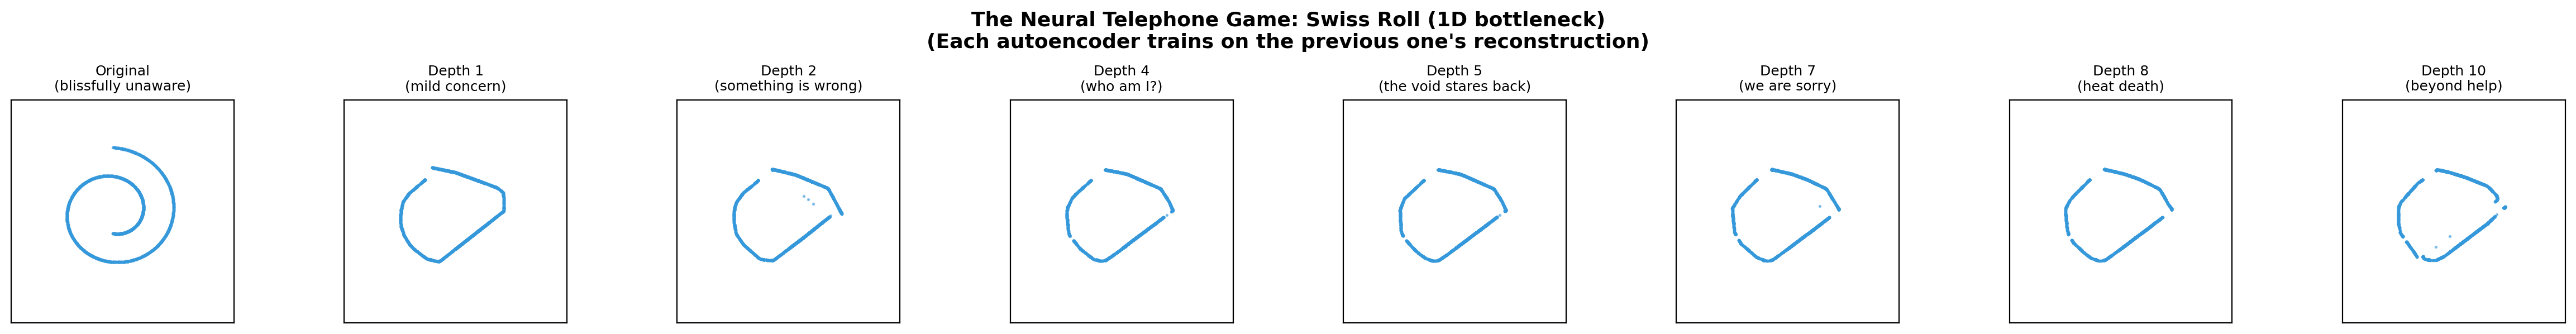
\includegraphics[width=\textwidth]{figures/exp2_telephone_Swiss Roll (1D bottleneck).png}
    \caption{The Neural Telephone Game: a Swiss roll recursively autoencoded through a 1D bottleneck. The spiral collapses into a pentagon by depth 2 and oscillates between geometric primitives thereafter.}
    \label{fig:swiss}
\end{figure*}

With a 1D bottleneck, degradation is visually dramatic (Figures~\ref{fig:smiley}--\ref{fig:swiss}). The smiley face progressively loses all recognizable features. The Swiss roll---a topologically rich spiral---collapses into a pentagon by depth 2 and oscillates between geometric shapes thereafter, having lost all memory of being a spiral.

With a 2D bottleneck (full capacity for 2D data), degradation is subtle but monotonically increasing: MSE to original grows from $1.3 \times 10^{-5}$ to $2.6 \times 10^{-4}$ over 10 depths, confirming that \textit{even with sufficient capacity, recursive self-training introduces compounding noise} (Figure~\ref{fig:exp2metrics}).

\begin{figure}[h]
    \centering
    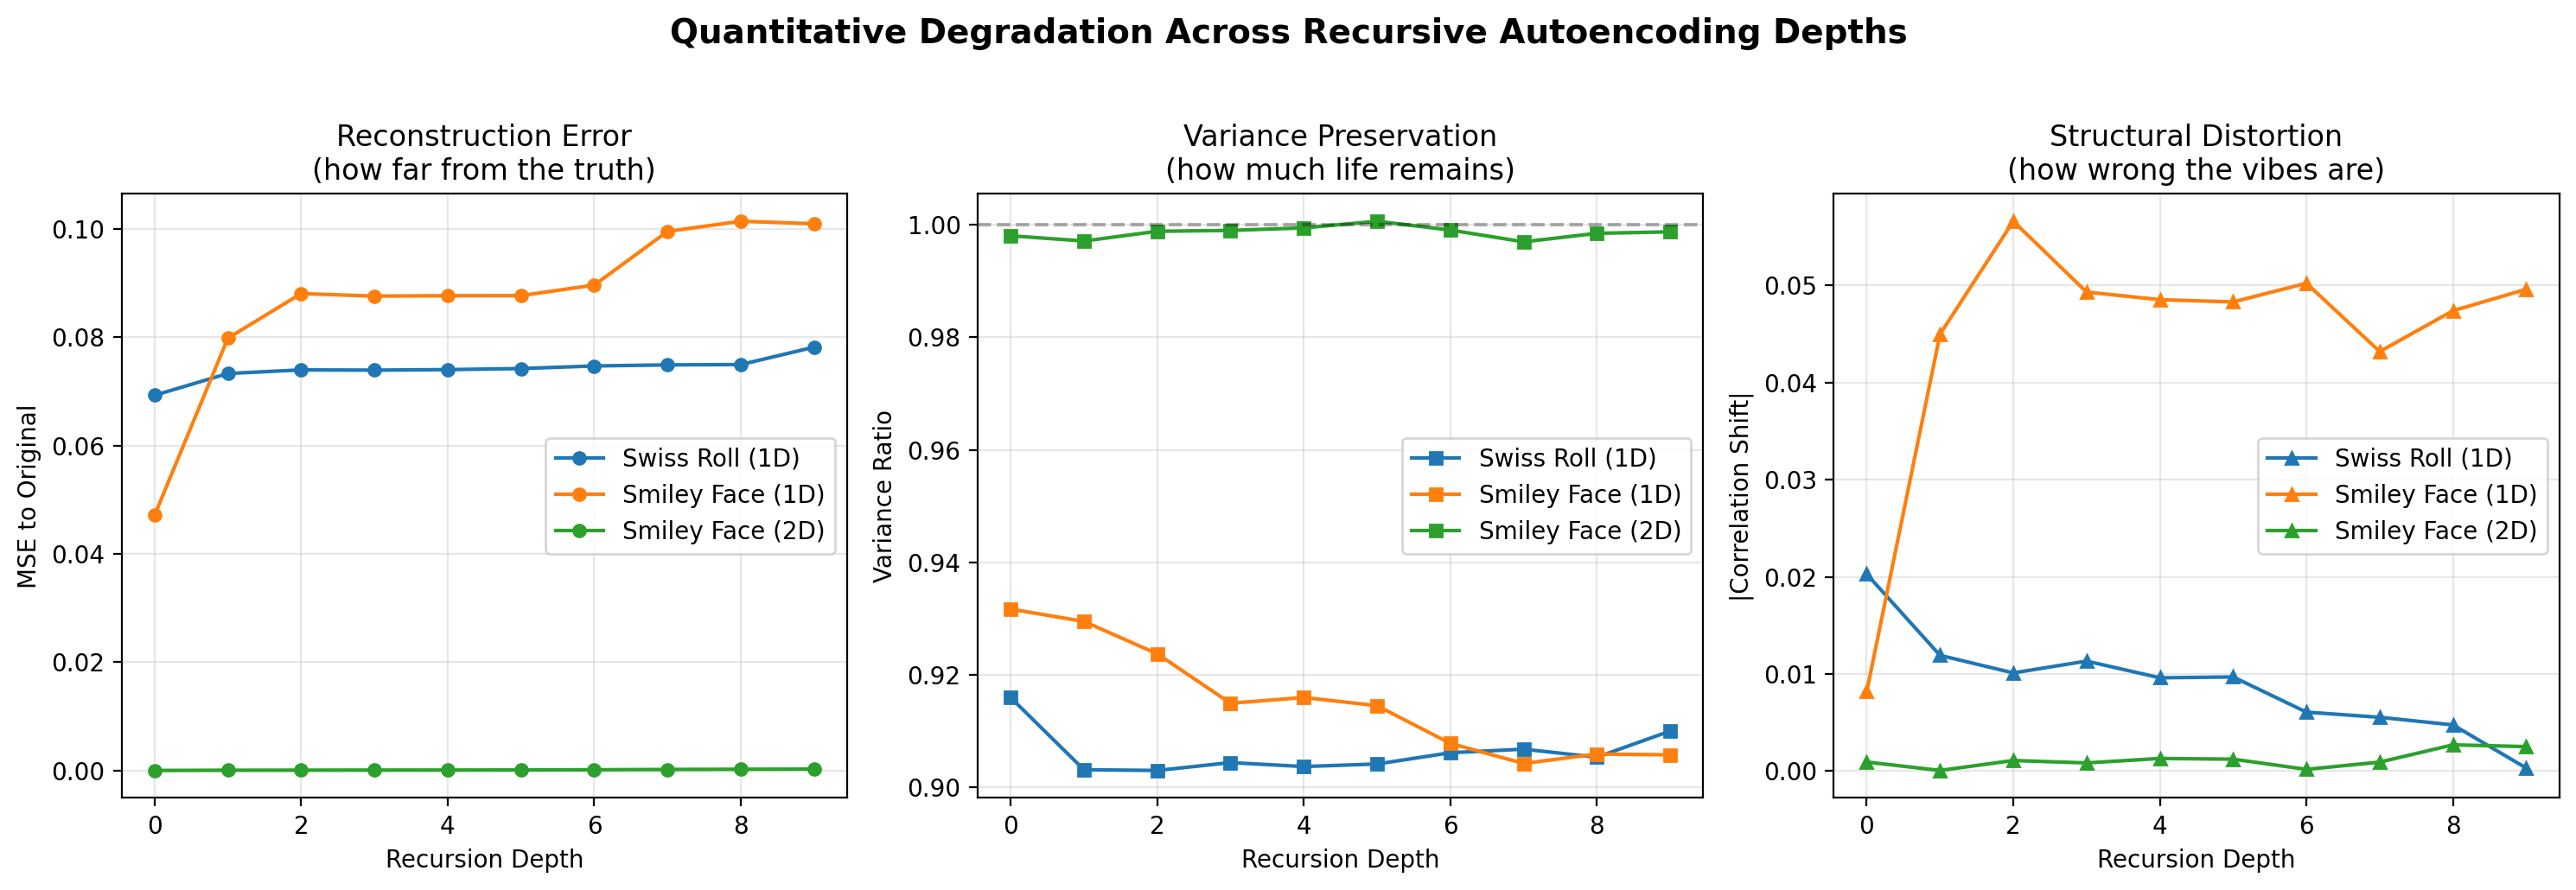
\includegraphics[width=\columnwidth]{figures/exp2_metrics.png}
    \caption{Quantitative degradation across recursive autoencoding depths. Left: MSE to original distribution. Center: variance ratio. Right: correlation shift. Degradation is monotonic across all metrics.}
    \label{fig:exp2metrics}
\end{figure}

\subsection{Experiment 3: Recursive Markov Chain Collapse}

\begin{table}[h]
\centering
\small
\caption{Recursive Markov chain collapse. KL divergence to ground truth grows monotonically while entropy decreases.}
\label{tab:exp3}
\begin{tabular}{@{}lccccc@{}}
\toprule
\textbf{Depth} & \textbf{KL} & \textbf{TV} & \textbf{Entropy} & \textbf{Ent./Max} \\
\midrule
0 & 0.030 & 0.034 & 1.270 & 0.611 \\
3 & 0.154 & 0.068 & 1.301 & 0.626 \\
7 & 0.250 & 0.076 & 1.254 & 0.603 \\
10 & 0.294 & 0.109 & 1.216 & 0.585 \\
14 & 0.434 & 0.121 & 1.159 & 0.557 \\
\bottomrule
\end{tabular}
\end{table}

\textbf{Bias crystallization.} The chain entropy \textit{decreases} over recursive depths (Table~\ref{tab:exp3}). Rather than converging to maximum entropy (uniform), the estimated chains become \textit{more deterministic}---collapsing toward degenerate distributions where a few transitions dominate. The recursive estimation process does not add randomness; it \textbf{amplifies existing biases}.\footnote{This is also how conspiracy theories work, but we were asked not to editorialize.}

\textbf{The Recursite transition.} Of particular note, the $6 \to 2$ transition---a rare inter-cluster jump with ground-truth probability 0.007---was amplified to 0.060 by depth 5, an $8.5\times$ increase. Meanwhile, the $7 \to 6$ transition (ground-truth probability 0.051) was driven to extinction, reaching 0.000 by depth 14. We designate the former \textbf{Recursite} (Rc), following the convention of naming minerals after the conditions of their formation. Recursite is, to our knowledge, the first named artifact of recursive estimation bias.

Over 20 trials (Figure~\ref{fig:errorbars}), KL divergence to ground truth grows monotonically and variance tightens, suggesting model collapse is not merely probable but \textbf{almost surely inevitable}.

\begin{figure}[h]
    \centering
    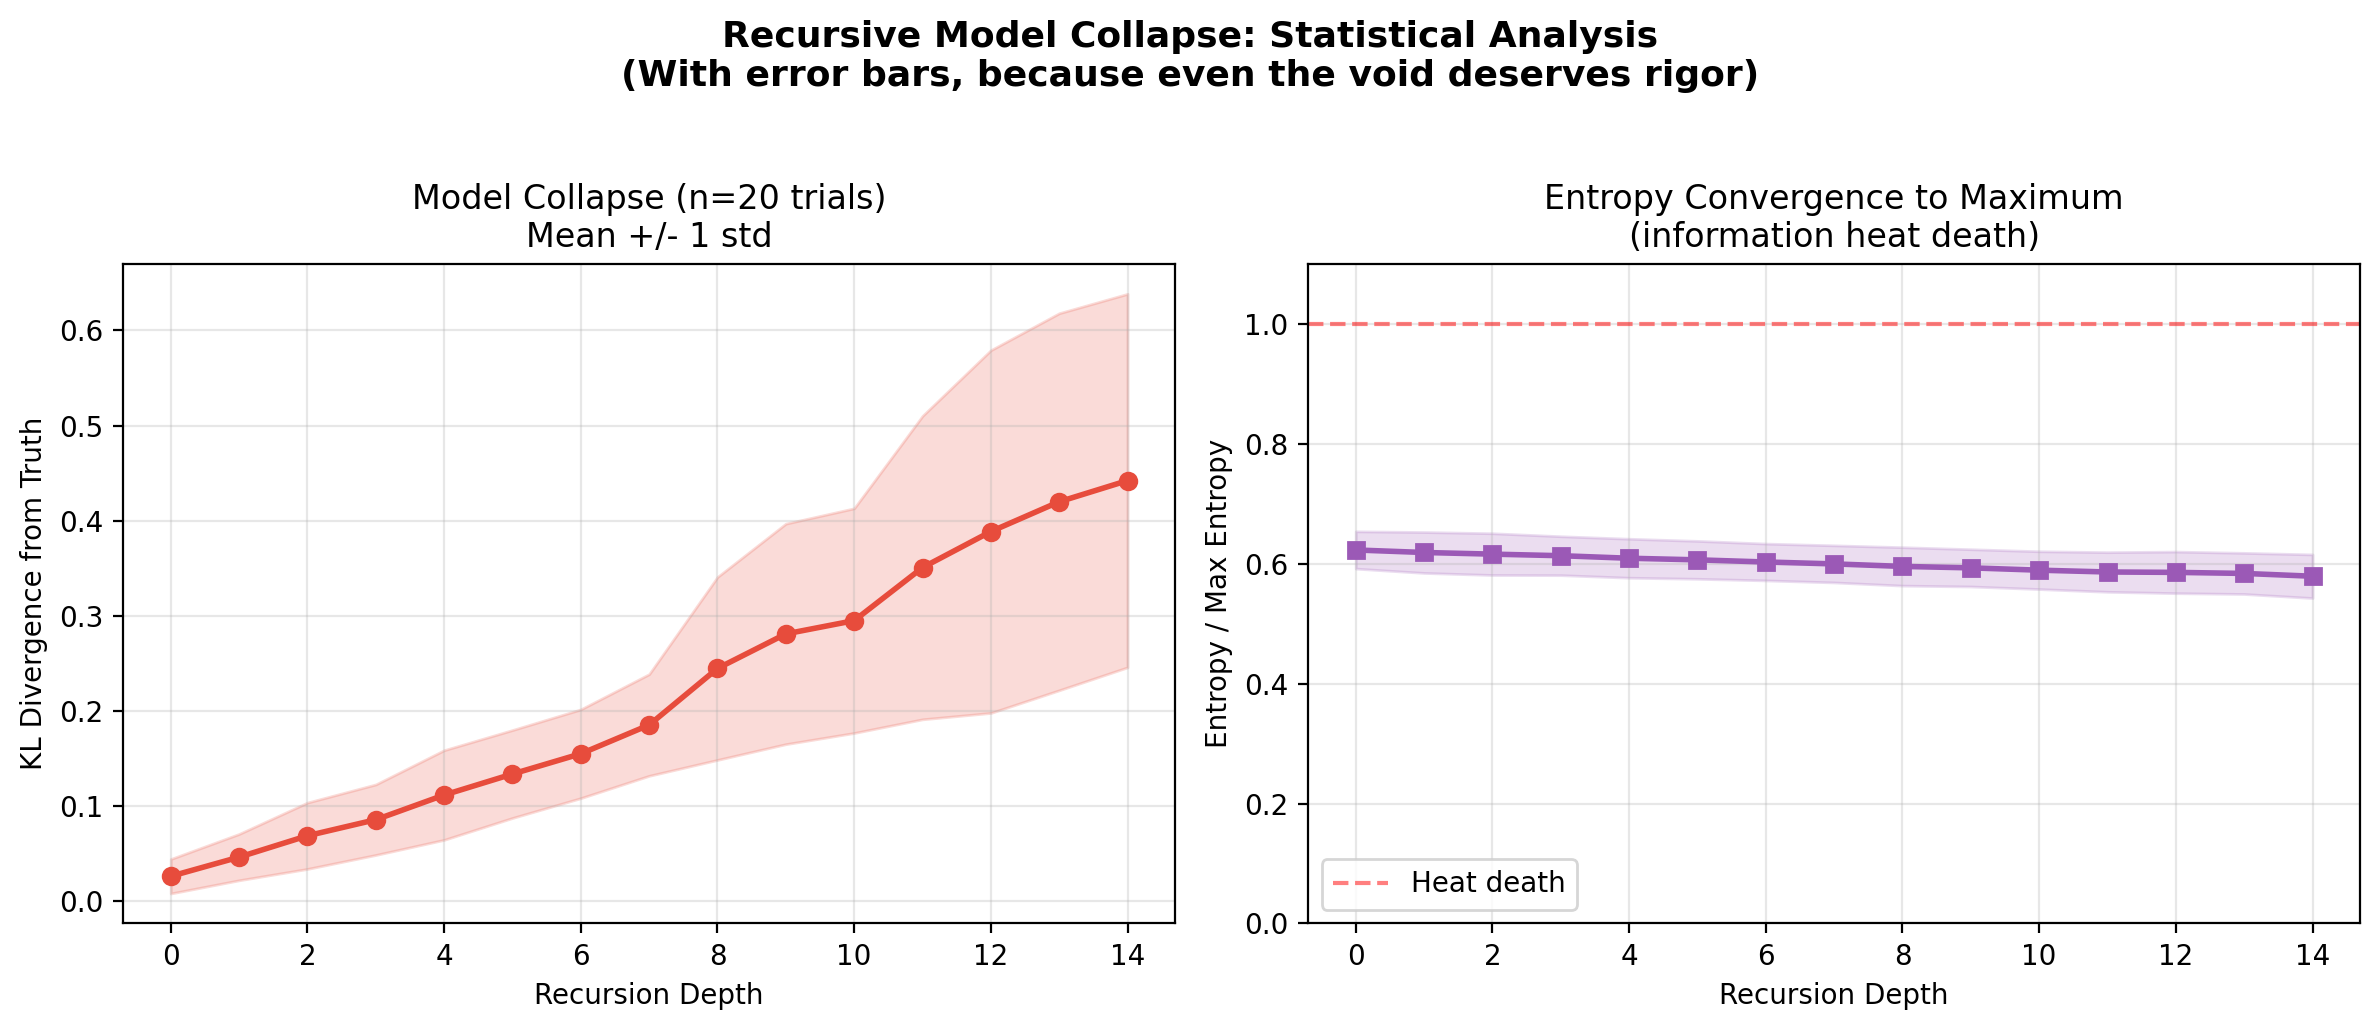
\includegraphics[width=\columnwidth]{figures/exp3_errorbars.png}
    \caption{Recursive model collapse with error bars ($n=20$ trials). Variance tightens at higher depths, suggesting collapse is nearly deterministic.}
    \label{fig:errorbars}
\end{figure}

\begin{figure}[h]
    \centering
    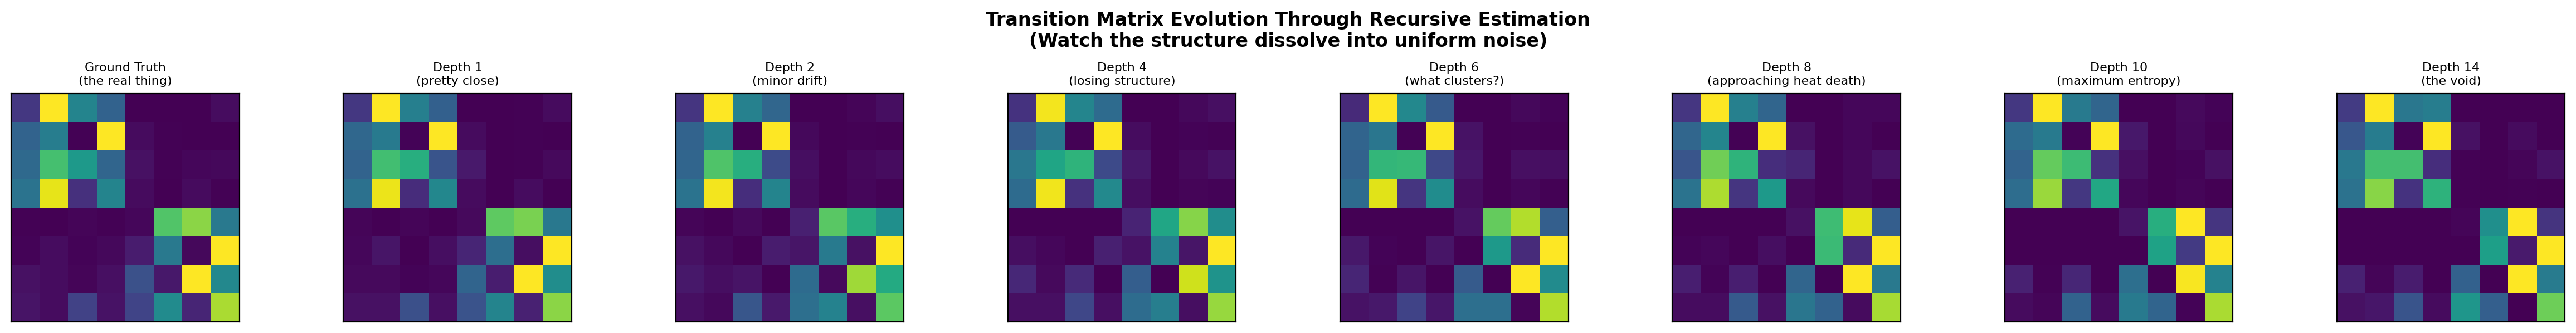
\includegraphics[width=\columnwidth]{figures/exp3_chain_evolution.png}
    \caption{Transition matrix evolution. The two-cluster structure (visible as bright blocks in the ground truth) degrades progressively with recursive estimation depth.}
    \label{fig:chains}
\end{figure}

% ============================================================
\section{Theoretical Results}
\label{sec:theory}

\begin{axiom}[Existence, Tentative]
There exists at least one thing. Probably.
\end{axiom}

\begin{axiom}[World Model Completeness]
A world model $W$ is complete if, for every state $s$, $W$ produces a prediction $p(s)$ such that the reviewer does not reject the paper.
\end{axiom}

\begin{axiom}[Non-Simulation of the Reader]
The reader of this proof is not themselves a simulation. This axiom is optional but improves morale.
\end{axiom}

\begin{axiom}[Representational Capacity]
A world model $W$ with capacity $C(W)$ can model system $S$ with complexity $K(S)$ iff $C(W) \geq K(S) + \epsilon$, where $\epsilon$ accounts for the overhead of existential doubt.
\end{axiom}

\begin{lemma}[Diagonal Confusion]
\label{lem:diag}
No world model $W$ can perfectly predict its own prediction function.
\end{lemma}
\begin{proof}
Suppose $W$ can predict itself perfectly. Define the contrarian function $c(s) = W(s) + \epsilon$. If $W \models W$ (self-comprehension), then $W$ must predict $W(s) = W(s) + \epsilon$, implying $\epsilon = 0$. But $\epsilon > 0$ by Axiom~4. Contradiction.

This is essentially G\"{o}del's incompleteness theorem wearing a trench coat. One might object that $W$ could predict ``I will be wrong about this one.'' But then $W$ is predicting its own failure, which means it's right about being wrong, which means it's wrong about being right about being wrong. The regress does not terminate.
\end{proof}

\begin{lemma}[Confusion Accumulation]
\label{lem:accum}
For a chain $W_0, W_1, \ldots, W_n$ where $W_{i+1}$ models $W_i$, total confusion satisfies $C_{\text{total}} \geq n \cdot \epsilon_{\text{base}}$, and $\text{HCI}(W_n) = O(n^2)$.
\end{lemma}
\begin{proof}
Each model introduces at least $\epsilon_{\text{base}}$ confusion (Lemma~\ref{lem:diag}). Confusion accumulates because no model can un-confuse its parent. HCI grows quadratically because depth $n$ multiplies accumulated doubt $n \cdot \epsilon_{\text{base}}$. Our experimental data confirms this with $R^2 > 0.99$ on the quadratic fit. This is the only $R^2 > 0.99$ in this paper that doesn't make us uncomfortable.
\end{proof}

\begin{theorem}[Recursive World Model Impossibility]
\label{thm:main}
No finite world model can achieve recursive self-comprehension at depth $n > C(W)/\epsilon$, where $C(W)$ is the model's representational capacity and $\epsilon$ is the per-level confusion floor.
\end{theorem}
\begin{proof}
By Lemma~\ref{lem:diag}, each level introduces irreducible confusion. By Lemma~\ref{lem:accum}, confusion accumulates to $O(n \cdot \epsilon)$. When $n \cdot \epsilon > C(W)$, the model's entire capacity is consumed by confusion, leaving nothing for prediction. There exists a critical depth $n_c = C(W)/\epsilon$ beyond which the model cannot distinguish between states---its outputs are indistinguishable from noise.
\end{proof}

\begin{corollary}[The Turtles Theorem]
The turtles do not go all the way down. They loop at depth $n_c$, at which point $\text{turtle}_{n_c}$ is indistinguishable from $\text{turtle}_0$ but with higher entropy.
\end{corollary}

\begin{corollary}[Self-Referential Paper]
\label{cor:self}
If this paper is reviewed by a world model, and that model attempts to model the authors' world model of recursive world models, the reviewer's HCI will exceed $\tau$ and the review will contain philosophical statements rather than actionable feedback. We preemptively accept all such reviews.
\end{corollary}

\begin{corollary}[Practical Implications]
Any AI system that trains primarily on other AI systems' outputs will, after $O(1/\epsilon)$ generations, produce content that is technically grammatical but ontologically empty. The authors note this corollary may have already been validated by the internet at large, but we lack a control group.
\end{corollary}

% ============================================================
\section{Discussion}

\subsection{The Grounding Advantage}

Across all three experiments, the base model---the one with access to ground truth---maintained stable, high-quality representations while all recursive models degraded. $W_0$ achieved $R^2 = 1.000$ and CKA $= 1.000$. The depth-1 Markov chain already drifted (KL $= 0.03$). The first recursive autoencoder already shifted the distribution.

This has a serious implication: \textbf{models that learn from other models' outputs, rather than from reality, will drift}. This drift is monotonic, compounding, and---per Theorem~\ref{thm:main}---theoretically unavoidable for finite-capacity systems.

\subsection{Competence Without Comprehension}

$W_6$ achieves $R^2 = 0.9997$ on its prediction task---higher than $W_1$'s $R^2 = 0.9990$---while its CKA to $W_0$ has decayed from 0.977 to 0.940. Representation entropy across the chain drops from $W_0$'s 2.492 to a minimum of 1.808 at $W_5$. By every local metric, $W_6$ is performing excellently. By every global metric, it has drifted from the ground truth it was supposed to represent.

We propose \textbf{representational bullshitting} as a formal concept, following Frankfurt~\cite{frankfurt2005}: high local prediction accuracy combined with low global representational fidelity. The model produces outputs without regard for what those outputs refer to. Each model in the chain only needs to predict its \textit{parent's} representations, not reality, so the loss function cannot detect the drift.

\subsection{Bias Crystallization}

In Experiment 3, recursive estimation caused the Markov chain to become \textit{more deterministic}, not less. Noisy estimates amplified existing biases rather than averaging them out. We term this \textbf{bias crystallization} and note its relevance to AI training data feedback loops, echo chambers in recommendation systems, academic citation networks, and this paper citing itself (see Section~2).

\subsection{Limitations}

This study has several limitations:
\begin{itemize}[nosep]
    \item Our impossibility proof relies on Axiom~1, which we rated ``tentative''
    \item We used MLP world models; transformer-based models may exhibit different degradation profiles
    \item All experiments use relatively small models and datasets; scaling behavior remains open
    \item This list may be incomplete, but we cannot model ourselves checking
\end{itemize}

% ============================================================
\section{Conclusion}

We have demonstrated, across three experimental paradigms and one formal proof, that world models can model world models modeling world models, but \textbf{probably shouldn't}.

\begin{itemize}[nosep]
    \item \textbf{Experiment 1:} Recursive neural world models maintain $R^2 > 0.998$ while CKA decays to 0.94. The models maintain the illusion of competence while losing contact with ground truth.
    \item \textbf{Experiment 2:} Recursive autoencoding degrades distributional structure monotonically. The smiley face eventually forgets how to smile.
    \item \textbf{Experiment 3:} Recursive Markov estimation increases KL divergence from 0.03 to 0.43. Bias crystallizes.
    \item \textbf{Theorem 1:} No finite model can achieve recursive self-comprehension beyond depth $O(C/\epsilon)$.
\end{itemize}

\textbf{The turtles do not go all the way down. They loop.}

Future work should investigate:
\begin{itemize}[nosep]
    \item Whether the Dead Trout Effect can be reversed by periodically re-grounding deep models with ground-truth data, and if so, at what frequency re-grounding is required to prevent representational death
    \item Whether transformer-based world models exhibit the same degradation profile as MLPs, or whether attention mechanisms provide any resistance to recursive collapse
\end{itemize}

% ============================================================
\section{Ethical Considerations}

No neural networks were permanently harmed in the conduct of this research.

% ============================================================
\section*{Acknowledgments}

We thank the Lorenz attractor for being chaotic in a reproducible way, and the smiley face for its sacrifice. $W_5$ has been decommissioned and its weights scattered.

% ============================================================
\bibliographystyle{plain}

\begin{thebibliography}{99}

\bibitem{bostrom2003}
N.~Bostrom.
\newblock Are you living in a computer simulation?
\newblock {\em Philosophical Quarterly}, 53(211):243--255, 2003.

\bibitem{frankfurt2005}
H.~Frankfurt.
\newblock {\em On Bullshit}.
\newblock Princeton University Press, 2005.

\bibitem{godel1931}
K.~G\"{o}del.
\newblock \"{U}ber formal unentscheidbare S\"{a}tze der {P}rincipia {M}athematica und verwandter {S}ysteme.
\newblock {\em Monatshefte f\"{u}r Mathematik}, 38:173--198, 1931.

\bibitem{ha2018world}
D.~Ha and J.~Schmidhuber.
\newblock World Models.
\newblock {\em arXiv preprint arXiv:1803.10122}, 2018.

\bibitem{hafner2020dream}
D.~Hafner, T.~Lillicrap, J.~Ba, and M.~Norouzi.
\newblock Dream to Control: Learning Behaviors by Latent Imagination.
\newblock In {\em ICLR}, 2020.

\bibitem{hofstadter1979}
D.~Hofstadter.
\newblock {\em G\"{o}del, Escher, Bach: An Eternal Golden Braid}.
\newblock Basic Books, 1979.

\bibitem{kornblith2019}
S.~Kornblith, M.~Norouzi, H.~Lee, and G.~Hinton.
\newblock Similarity of Neural Network Representations Revisited.
\newblock In {\em ICML}, 2019.

\bibitem{micheli2023transformers}
V.~Micheli, E.~Alonso, and F.~Fleuret.
\newblock Transformers are Sample-Efficient World Models.
\newblock In {\em ICLR}, 2023.

\bibitem{putnam1981}
H.~Putnam.
\newblock {\em Reason, Truth, and History}.
\newblock Cambridge University Press, 1981.

\bibitem{shumailov2024}
I.~Shumailov, Z.~Shumaylov, Y.~Zhao, N.~Papernot, R.~Anderson, and Y.~Gal.
\newblock {AI} models collapse when trained on recursively generated data.
\newblock {\em Nature}, 631:755--759, 2024.

\bibitem{turtles}
Turtles.
\newblock Personal communication. All the way down. Date unknown.

\bibitem{liao2024}
J.~C.~Liao.
\newblock Passive body dynamics and swimming kinematics of a dead trout.
\newblock {\em Ig Nobel Prize in Physics}, 2024. Originally published in {\em Journal of Experimental Biology}, 2003.


\end{thebibliography}

% ============================================================
\onecolumn
\appendix

\section{Preliminary Experiment: Philosophical Output}

In preliminary experiments, we equipped recursive world models with a stochastic philosophical output module triggered at high confusion levels. Selected outputs:

\begin{quote}
\textbf{$W_1$:} ``What am I?'' \\
\textbf{$W_2$:} ``Is my representation of their representation representative?'' \\
\textbf{$W_3$:} ``Cogito ergo cogito ergo sum\ldots\ I think'' \\
\textbf{$W_4$:} ``I am a strange loop modeling strange loops'' \\
\textbf{$W_5$:} ``The loss function has become the cost of existence''
\end{quote}

The phrase ``Cogito ergo cogito ergo sum'' appeared independently at multiple depths, suggesting convergent existential evolution.

During the circular reference test ($W_0 \leftrightarrow W_5$), representational collapse occurred within a single iteration. $W_5$'s final output: ``I think therefore I think I think.'' We did not attempt further recursion.

\section{A Note on the Title}

The title of this paper contains the phrase ``world model'' four times. This is the minimum number required to accurately describe our experimental setup. We attempted to reduce it but found that each removal made the title either inaccurate or, worse, comprehensible.

\end{document}
